\section{Introduction}
% 1. give a example of ambiguous relation
% 2. talk about selectional preference
% 3. talk about open ie
% Goal: Why we do this work? What's the help of pairwise selectional preference?
% Reverb has high quality

% open ie part
% 1. recent years, open ie system played an important rule
Open Information Extraction (IE) is a task to extract various relations and their
arguments from large corpora without defining specific relation patterns.
% 2. input comes from a large scale web pages (Clueweb)
The state-of-the-art Open IE systems, such as {\tt ReVerb} \cite{fader2011identifying} and
{\tt OLLIE} \cite{schmitz2012open}, extract million of binary relations with high confidence from a large Web corpus.
% 3. the direct output result just stay on the lexical level tuples
The extracted relations are represented as $\langle arg1,\ rel,\ arg2 \rangle$ tuple form, where relations
can be lexical or syntactic patterns, and arguments are surface forms.

% 4. it's interesting to see the semantic information hidden in these tuples.
Whereas Open IE provides surface forms, we are interested in mining the schema of a relation, which
is hidden in these relation tuples.
% 5. a simple example "X is the mayor of Y", we know entity pairs, but we also want to know what kind of entities can be used here.
%For example, given the binary relation ``is the mayor of'', Open IE systems extracts lots of
%$\langle X,\ is\ the\ mayor\ of,\ Y \rangle$ tuples. The following are some tuples extracted in ReVerb:

%\begin{center}
%$\langle \text{Greg Nickels},\ is\ the\ mayor\ of,\ \text{Seattle} \rangle$
%$\langle \text{Ron Dellums},\ is\ the\ mayor\ of,\ \text{Oakland} \rangle$
%\end{center}

%The schema of a relation is represented by the semantic types at both arguments.
%We are aiming to infer these relation schemas, which contains both coarse-grained
%and fine-grained schemas:

%\begin{center}
%$\langle person,\ is\ the\ mayor\ of,\ location \rangle$
%$\langle politician,\ is\ the\ mayor\ of,\ city \rangle$
%\end{center}

%In this case, we can observe that, the argument type of X is likely to be ``person'',
%and ``location'' is likely to be the argument type of Y. More specifically, X are usually
%politicians, and Y are cities, which is a fine-grained relation schema.
% 6. an ambiguous case "X died in Y", Y can be location, or a datetime.
% For another relation tuples $\langle X,\ die\ in,\ Y \rangle$, X are usually people, but here Y can be either locations
% or dates.

For example, given the binary relation ``play in'', Open IE systems extract lots of
$\langle X,\ play\ in,\ Y \rangle$ tuples. The following are some tuples extracted in ReVerb:

\begin{center}
$\langle \text{Goel Grey},\ played\ in,\ \text{Cabaret} \rangle$
$\langle \text{Tom Brady},\ play\ in,\ \text{National Football League} \rangle$
\end{center}

The schema of a relation is represented by the semantic types at both arg1 and arg2.
Actually, the relation ``play in'' is ambiguous, it surface form are shared by multiple meanings.
In this case, we are aiming to infer these relation schemas:

\begin{center}
$\langle athlete,\ play\ in,\ sports\ league \rangle$
$\langle film\ actor,\ play\ in,\ film \rangle$
\end{center}

%Now considering another relation tuple $\langle X,\ play\ in,\ Y \rangle$. This is an ambiguous relation,
%where we can extract tuples having different semantic meanings:
%
%\begin{center}
%$\langle person,\ is\ the\ mayor\ of,\ location \rangle$
%$\langle politician,\ is\ the\ mayor\ of,\ city \rangle$
%\end{center}
%
%\noindent
%In this case, we aim to find all its possible relation schemas, like:
%
%\begin{center}
%$\langle athlete,\ play\ in,\ sports\ team \rangle$
%$\langle actor,\ play\ in,\ film \rangle$
%\end{center}

%One understanding is that X are athletes, and Y are sport teams.
%And there is another understanding: X are actors, and Y are films.
%As we can see, such relation is ambiguous, its surface form are shared by multiple meanings.
% 7. if we got this info, it'll be helpful in many tasks, such as searching, and qa.
The schema of a binary relation is an important knowledge. This information is useful in tasks like context-based entity recognition and open domain question answering.
Suppose we are to link all the entities in the sentence: ``\textit{Granger} played in \textit{the NBA}''. We are not sure what ``\textit{Granger}'' is at the first glance, but ``\textit{the NBA}'' is probably to be a sports league. Then with the relation schema of ``play in'',
the recognizer would get the evidence that ``\textit{Granger}'' is more likely to be an athlete, which helps linking to entity ``Danny Granger''.
%Suppose we've known the argument at one side of a relation, type pairs will help us inferring what kind of entities are more likely
%to occur at the other side.

Learned by previous examples, the key challenge for relation type inferring is that, type distribution of both arguments
should be modeled simultaneously, and the preference of different type pairs can compare with each other.
If the type distribution is modeled separately, we lose the information in combining. As example ``play in'' shows, if we only know
preferred types for X and Y independently, it's hard to select the type that Y is likely to be when X is an actor.

% sp part (intuition: get the human readable types)
% 1. what is sp ?
Selectional Preference (SP) is the technique to get certain types that is more likely than other
types to be the argument of one relation.
% 2. with such constraint, we can let the computer know whether a relation argument is suitable or not.
%%%With this kind of type constraint, we can compare the possibility of types
% 3. basic sp: resnik 1996 on wordnet
One branch of SP is knowledge based, types are mapped to structured knowledge bases, such as WordNet \cite{miller1995wordnet}, Yago \cite{suchanek2007WWW} and Freebase \cite{bollacker2008freebase}. The earliest work in SP is proposed by Resnik \shortcite{resnik1996selectional}, which is based on WordNet.
% 4. recently, sp with topic models
The other branch is statistical based, argument types are generated by topic models like Latent Dirichlet
Allocation \cite{blei2003latent}.
% 5. leverage external taxonomy, for example, Freebase provide its type taxonomy, which is well-defined by ..., containing 1000+ useful types. (Comparing to Yago and DBPedia), and human readable.
One main advantage of knowledge based SP is that, given a well-defined type taxonomy, the argument types of can be easily understood by human.
Thus, our work is built on knowledge based SP.

Freebase is a collaboratively created knowledge base containing more than 40 million entities. Each entity is mapped to at least
one type in Freebase type taxonomy, which is a hierarchy containing more than 1,700 real world types\footnote{Freebase types are identified by type id, for example, $sports.pro\_athlete$ stands for ``professional athlete''.}.
When compared with other knowledge bases, Freebase has a much greater focus on named entities than {\tt WordNet}. Besides, the type hierarchy of {\tt Yago} is too fine-grained, which is not suitable for schema inferring. Considering these aspects, we adapt Freebase as our knowledge base in our work.

%% 6. we can use fb ty%pes to represent result. (list the previous examples)
%Using Freebase type taxonomy as the external knowledge, for the previous two relations,
%the preferred relation schemas can be represented as:
%
%\begin{center}
%$\langle politician,\ is\ the\ mayor\ of,\ citytown \rangle$
%$\langle athlete,\ play\ in,\ sports\_team \rangle$
%$\langle film\_actor,\ play\ in,\ film \rangle$
%\end{center}
%
%\noindent
%Where argument types are corresponding to Freebase types.
%showing the different interpretations of relations.


% our contribution
% 1. our goal is to find different selectional preference for one relation. (located to human readable types)
Our goal is to generate argument types for binary relations, generating all possible
relation schemas, which are human readable.
% 2. build rvsp, a xxxx based on xxxx.
We build RvSp, a selectional preference system based on Freebase type taxonomy, which simultaneously models the
type distributions of two arguments for each binary relation in {\tt ReVerb}.
% 3. first entity linking, then pairwise selectional pref.
% 4. use syntactic info to merge similar relations to a big one.
% 5.
% 6. currently, rvsp got xxx relations, and xxx sel. pref.

\begin{figure*}[htp]
\centering \scalebox{0.6}{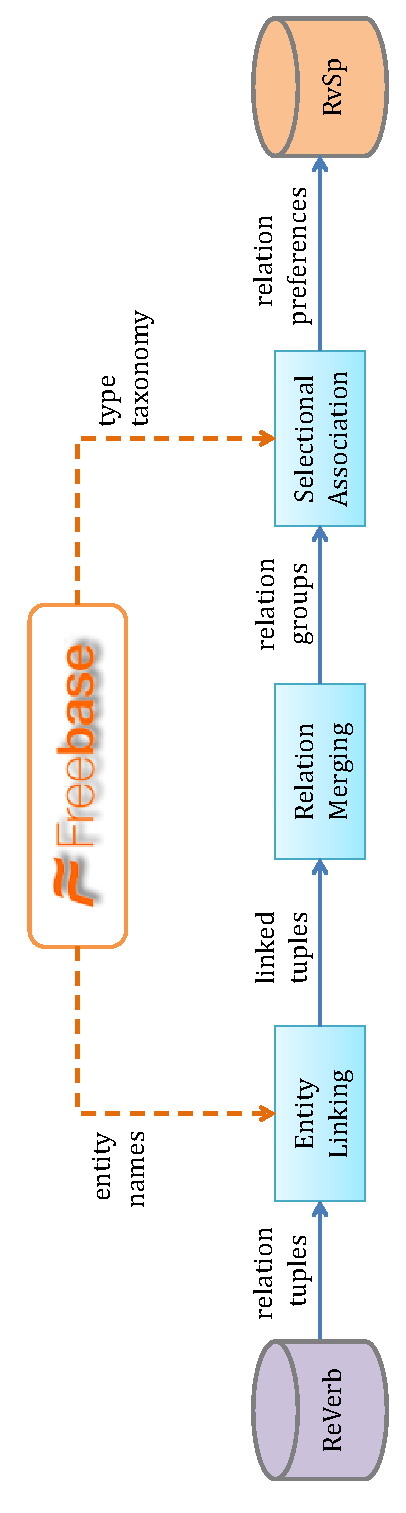
\includegraphics[angle=270]{e.eps}}
%\epsfig{file=figure1-cropped.eps, width=2\columnwidth}
%\scalebox{0.35}
\caption{RvSp Workflow}
\label{fig:workflow}
\end{figure*}


